
\chapter{Resonance Search and Results}

The following chapter will discuss the details and results from a resonance 
search conducted on the 2015 engineering run data.  This includes a discussion
of the procedure used to determine if a significant resonance was observed at 
a given $A'$ mass hypothesis and the statistical formalism used to set an upper
limit on both the signal and $A'$ coupling strength.

This analysis makes use of
the unblinded portion of the engineering run data ($\sim$ 10\% of total data) 
which amounts to 
a luminosity 74 nb$^{-1}$.  A blind search for a resonance using the procedure 
outlined in this chapter and making use of the full 2015 engineering run 
dataset is expected to be completed in the Summer of 2016.

\section{Searching for a Resonance}

If a heavy photon does indeed exist and has a mass that is within the acceptance
of the HPS detector, it will appear as a resonance above the copious QED trident
invariant mass distribution.  Such a signal is expected to be Gaussian in nature, 
centered on the mass of the $A'$ and with a width equal to the experimental
mass resolution. With this in mind, the invariant mass distribution measured by
HPS (see section 4 and Fig. \ref{fig:mass_distribution}) will serve as the 
starting point for this analyses.
\begin{figure}[t]
    \centering
    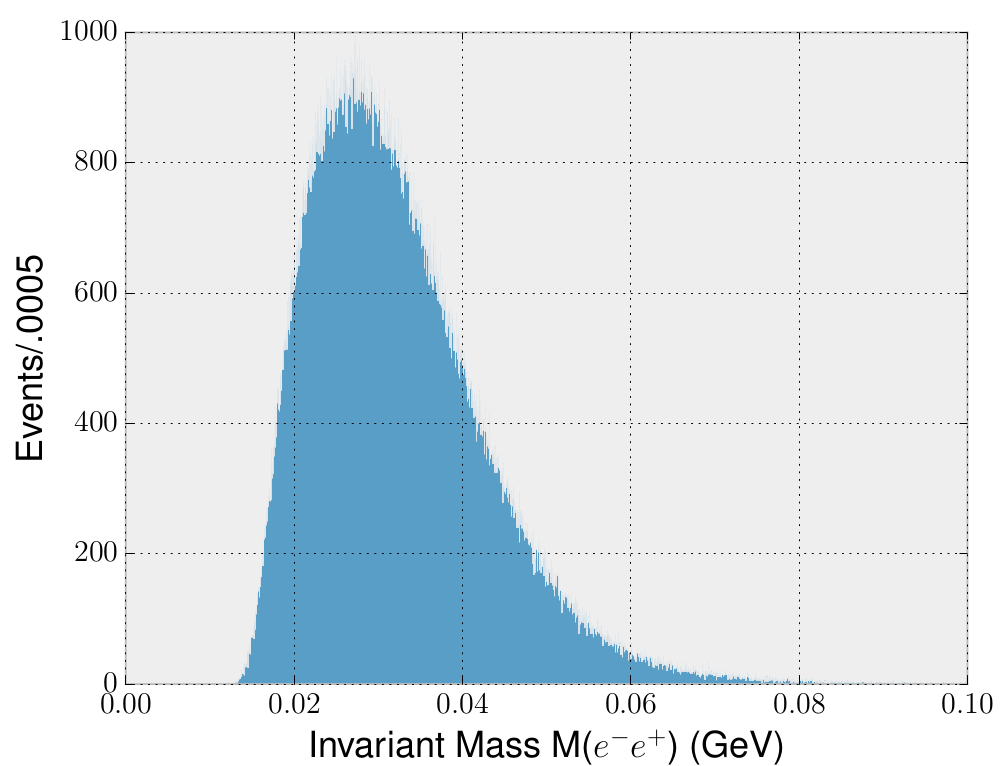
\includegraphics[width=1.0\textwidth]{images/invariant_mass_final.png}
    \caption{The Heavy Photon Search $e^+e^-$ invariant mass distribution after
             the final event selection has been applied.  The mass distribution
             will serve as the starting point for the resonance search.}
    \label{fig:mass_distribution}
\end{figure}

\subsection{Maximum Likelihood Fit}

Since the mass of the $A'$ is unknown a priori, the 
$e^+e^-$ invariant mass spectrum needs to be scanned for any significant peaks.
Customarily, a search for a resonance is performed within a
window constructed around the mass hypothesis of interest.  Within the window, $A'$ 
signal events are expected to appear as a Gaussian resonance, 
$\phi(m_{e^+e^-} | m_{A'}, \sigma_{m_{A'}})$, centered at
the mass hypothesis, $m_{A'}$ and with a width, $\sigma_{m_{A'}}$, equal to the
 measured mass resolution of
the experiment.  The distribution of background events within the same window
can be modeled by a polynomial, $p(m_{e^+e^-} | t_j)$, with coefficients $t_j$.  Estimating the 
signal yield, $\mu$, within
the window, as well the background normalization, $B_{total}$ and shape, can be
done by the method of maximum likelihood.  The theoretical formalism
used to do this will be outlined here but a detailed discussion can be found in
\cite{Cowan:2010js}.

Assume the events within the window are binned as $\mathbf{n} = (n_{1}, ... n_{i})$.
Furthermore, assume the center of the $i$th bin is given by $b_i$ and has a width
equal to $\epsilon$. 
The expectation value of the $i$th bin is given by 
\begin{equation}
    E[n_i] = S_{i} + B_{i}
\end{equation}
where 
\begin{equation}
    S_{i} = \mu \int_{b_i - \epsilon/2}^{b_i + \epsilon/2} \phi(m_{e^+e^-} | m_{A'}, \sigma_{m_{A'}}) d (m_{e^+e^-})
\end{equation} 
\begin{equation}
    B_{i} = B_{total} \int_{b_i - \epsilon/2}^{b_i + \epsilon/2} p(m_{e^+e^-} | t_{j}) d (m_{e^+e^-}).
\end{equation}
Denoting the nuissance parameters as $\theta = (B_{total},  t_{j})$, an estimation
of $\mu$ and $\theta$ can be obtained by finding the parameters $\hat{\mu}$ and
$\hat{\theta}$ which maximize the Poisson likelihood function, $\mathcal{L}$, within
the window
\begin{equation}
    \mathcal{L}(\mu, \theta) = \prod_{k=1}^{i} \frac{(S_{k} + B_{k})^{n_k}}{n_{k}!} e^{-(S_{k} + B_{k})}. 
\end{equation}
In the case where the invariant mass is scanned for a resonance, the Poisson 
likelihood function is maximized within each window corresponding to different
$A'$ mass hypothesis. This yields estimators for the signal yield and nuissance
parameters at each $A'$ mass hypothesis which are used to determine if a significant 
resonance was found.

\subsection{Likelihood Ratio}

When searching for a resonance above a background distribution, it is 
necessary to discriminate between two scenarios:
\begin{itemize}
    \item The background only or null hypothesis, $H_{0}: \mu = 0$.
    \item The signal+background hypothesis or alternative, $H_{1}: \mu > 0$.
\end{itemize}
Establishing whether the signal+background model is significantly different 
from the background only model is typically done using the profile likelihood
ratio
\begin{equation}
    \lambda(\mu) = \frac{\mathcal{L}(\mu, \hat{\hat{\theta}})}{\mathcal{L}(\hat{\mu}, \hat{\theta})}
    \label{eqn:likelihood_ratio}
\end{equation}
where $\hat{\hat{\theta}}$ is the conditional estimator for the nuissance parameters 
obtained by maximizing the Poisson likelihood assuming that the null or 
background only hypothesis is true i.e. $\mu = 0$.
As can be seen from \ref{eqn:likelihood_ratio}, 
if the estimator of the signal yield, $\hat{\mu}$, is compatible (incompatible) with the background
only hypothesis the likelihood ratio will tend to 1 (0).

A more convenient test statistic is the log likelihood ratio defined as
\begin{equation}
    q_0 = \begin{cases}
            -2 \ln \frac{\mathcal{L}(0, \hat{\hat{\theta}})}{\mathcal{L}(\hat{\mu}, \hat{\theta})} 
            & \hat{\mu} > 0 \\
             0  & \hat{\mu} < 0
        \end{cases}
\end{equation}
According to Wilkes theorem \cite{Wilks:1938dza}, in the large sample limit, the test statistic
$q_0$ is asymptotically $1/2\chi^2$ \footnote{The 1/2 comes from the fact that only
signal yields greater than 0 are being considered. See \cite{Cowan:2010js} for a 
more detailed explanation.} distributed with degrees of freedom equal to the
difference in parameters between the two models being tested.  In our current case, 
the number of degrees of freedom is one, since the signal yield is the only 
parameter that does not appear in
the background only model.

Quantifying how extreme the observation is can be done by calculating a $p$-value as
\begin{equation}
    p = \int_{q_{0,obs}}^{\infty} f(q_{0} | 0) dq_{0}.
\end{equation} 
This is shown graphically on Fig. \ref{fig:p_value}.  Typically, the observed 
p-value is
\begin{figure}[t]
    \centering
    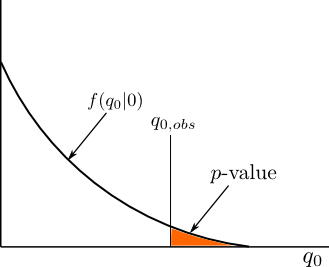
\includegraphics[width=.5\textwidth]{images/p_value.png}
    \caption{Graphical representation of a p-value.}
    \label{fig:p_value}
\end{figure}
compared against a significance level $\alpha$.  The significance level denotes
the probability of incorrectly rejecting the null hypothesis in favor of the 
alternative (type-I error).  In other words, it denotes the probability of there
being a statistical fluctuation in the background large enough to mimic a signal.  
If a $p$-value is 
found to be less than $\alpha$, the measurement is claimed to be significant. 
Typically, in particle 
physics, an $\alpha$ on the order of $3 \times 10^{-7}$ (5$\sigma$) is required
to claim discovery of new phenomena.  This means that there is a 1 in 
about 3.5 million chance that the observation is due to a fluctuation in the background.

\subsection{The Look-Elsewhere Effect}

As discussed in previous section, a result is determined significant if the 
$p$-value is smaller than some pre-determined threshold, $\alpha$.  However, 
when performing multiple test, as is the case when scanning a mass distribution
for a resonance, an observation with a $p$-value that is as extreme as $\alpha$
is bound to occur at a rate of $n\times\alpha$ where $n$ is the number of measurements.
This phenomena is known as the ``Look-Elsewhere Effect'' (LEE)
and needs to be taken into account through a correction to the ``local'' $p$-value
observed at each mass hypothesis.

Assuming that only a single heavy photon can be observed within the HPS invariant
mass distribution, the correction can be estimated using a large number
of pseudo-data sets and generating the distribution 
$f(q_{0, max} | 0)$ composed of the largest $q_{0}$ (i.e. smallest $p$-value)
from each of the invariant mass scans.
%The distribution $f(q_{0, max} | 0)$ can
%be derived by running a large number of pseudo-experiments and then calculating
%the $p$-value as was explained previously.
However, generating a distribution of $f(q_{0, max} | 0)$ that would allow 
an estimation of a ``global''  
$p$-value (i.e. local $p$-value after correction) down to the level of 5$\sigma$ with any accuracy would 
require running $\sim 10^{6}$ pseudo experiments.  Generating so many pseudo-data 
sets if often not feasible within a reasonable time. 

Instead, the smallest
$p$-values obtained from a modest number of pseudo-experiments were
ranked and the corresponding quantile was calculated \cite{Gross:2010qma}.  
A mapping from a local 
$p$-value to a global $p$-value is then created.  For this analysis, such a mapping
was created using 10,000 toys and is shown on Fig. \ref{fig:global_p_value}.  
\begin{figure}[t]
    \centering
    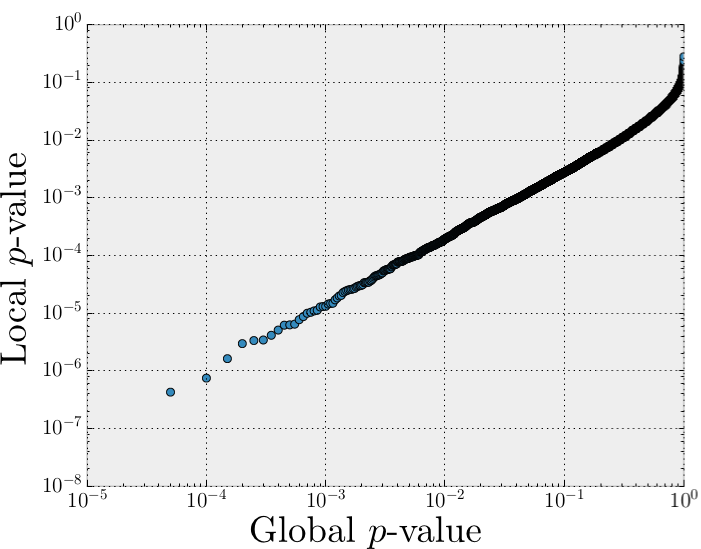
\includegraphics[width=.8\textwidth]{images/global_p_value_map.png}
    \caption{Mapping between local and global p-values.}
    \label{fig:global_p_value}
\end{figure}
As can be seen from the figure, a 
local $p$-value equal to 0.05 corresponds to a global $p$-value of $\sim$ 0.5.

%\section{Optimization of Fit Procedure}

%\subsection{Pseudo Data Sets}

%Pseudo data sets are needed to understand fitting systematics and to optimize
%both
%the fit function and window size.  In order to obtain an invariant mass probability
%density function (PDF) that describes the data, smoothing algorithm 353 QH 
%\cite{Friedman:1974vj} was
% What smoothing algorithm was used? Why? Was a K-S test used to make sure the
% resulting PDF matched the data set?
%applied the unit normalized final invariant mass MC distribution.  The resulting
%PDF after smoothing (blue line) overlayed over the MC distribution it was generated 
%from is shown on Fig. \ref{fig:smooth_pdf}.
%\begin{figure}[b]
%    \centering
%    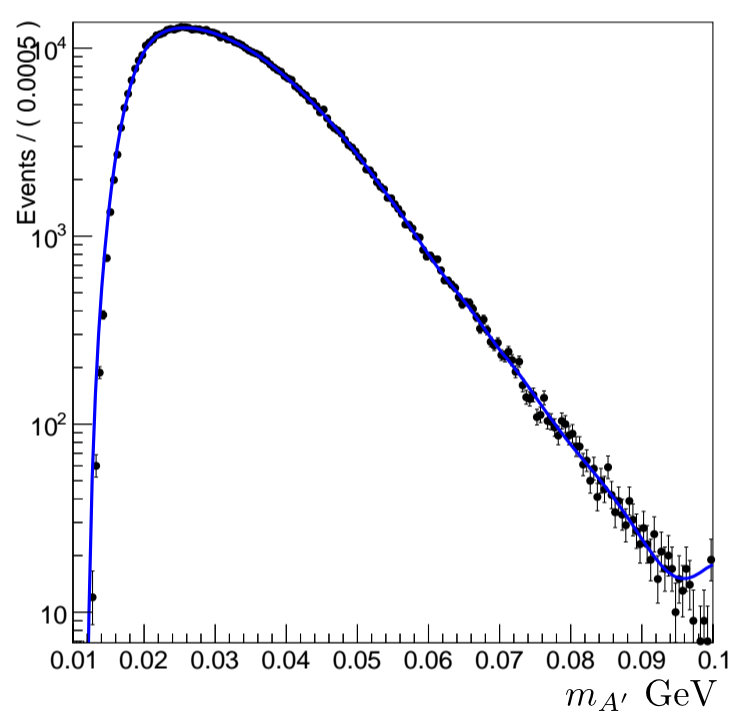
\includegraphics[width=0.7\textwidth]{images/smooth_pdf.png}
%    \caption{Probability density function obtained by applying a smoothing algorithm 
%             to the Heavy Photon Search Monte Carlo invariant mass distribution.}
%    \label{fig:smooth_pdf}
%\end{figure}
 

%Events were sampled from the PDF between 0 and 100 MeV with the total number of
%% What kind of sampling algorithm was used? 
%events, 579336, chosen to match the number observed in data.  The resulting
%pseudo data is binned to match the data distributions with the expectation
%value of each bin Poisson distributed.

\subsection{Results}

The resulting local $p$-values from a resonance search conducted in the range 
between 20 MeV and 75 MeV are shown on Fig. \ref{fig:local_p_values}. 
The most significant signal
was found at a mass of 28.525 MeV and has a local p-value of $4 \times 10^{-3}$.
After correcting for the LEE, the corresponding global p-value is 
$\sim 10\%$.
\begin{figure}[t]
    \centering
    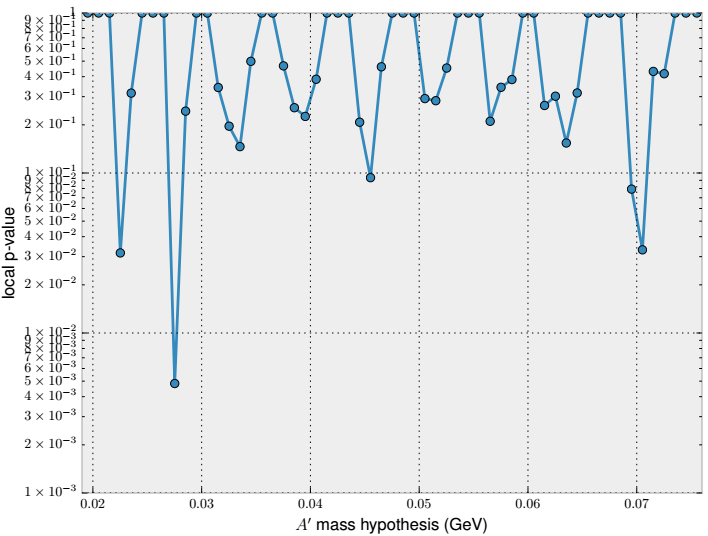
\includegraphics[width=.8\textwidth]{images/final_p_values.png}
    \caption{Resulting $p$-values from a resonance search for an $A'$ across the
    invariant mass spectrum.}
    \label{fig:local_p_values}
\end{figure}

\section{Setting Upper Limits on the Signal Yield}

Since no significant resonances were found, a 90\% confidence upper limit on the number
of signal events at each mass hypothesis was set.  For the purpose of setting
an upper limit, the likelihood ratio is inverted.  The statistic used
to set an upper limit is then
\begin{equation}
    q_{\mu} = \begin{cases}
        -2 \ln \frac{\mathcal{L}(\mu, \hat{\hat{\theta}})}{\mathcal{L}(0, \hat{\hat{\theta}})} 
            & \hat{\mu} < 0 \\
        -2 \ln \frac{\mathcal{L}(\mu, \hat{\hat{\theta}})}{\mathcal{L}(\hat{\mu}, \hat{\theta})} 
            & 0 \leq \hat{\mu} \leq \mu \\
             0  & \hat{\mu} > \mu
        \end{cases}
\end{equation}
with the corresponding $p$-value being given by
\begin{equation}
    p = \int_{q_{\mu,obs}}^{\infty} f(q_{\mu} | \mu) dq_{\mu}.
\end{equation}
In order to find the upper limit, the test above is carried out over a range of
signal yields until a $p$-value of 0.1 (90\% confidence) is found. The value of
$\mu$ found in this way
is often referred to as the unconstrained limit. The resulting 
unconstrained upper limits are shown in blue on Fig. \ref{fig:upper_limit}. 
\begin{figure}[t]
    \centering
    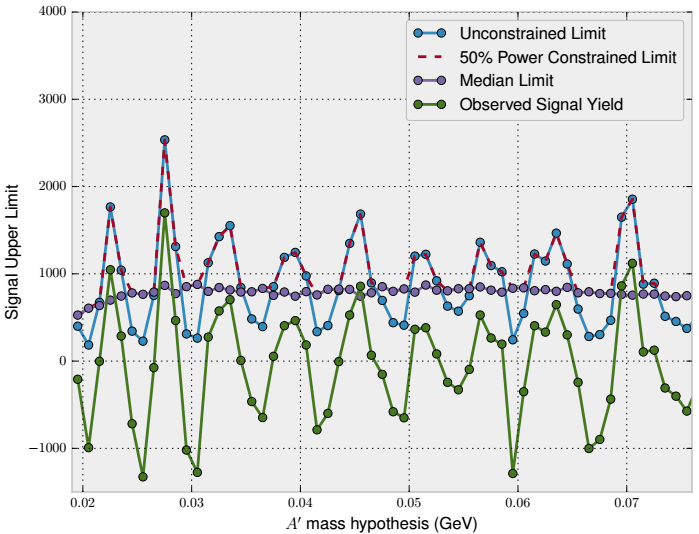
\includegraphics[width=.8\textwidth]{images/upper_limits.png}
    \caption{Upper limits on the signal yield at each mass hypothesis.}
    \label{fig:upper_limit}
\end{figure}

As shown in green on Fig. \ref{fig:upper_limit}, it is often the case that the
estimator for the signal yield at a given mass hypothesis is close to zero or
even negative.  As a result, the upper limit of those measurements will be small
relative to the background only hypothesis. This leads to a lack of 
sensitivity to a signal measurement at those mass hypothesis.

In such cases, a 50\% power-constrained upper limit on the signal is set
\cite{Cowan:2011an}.
At each mass hypothesis, a distribution of signal upper limits is generated from
background only pseudo-data sets and the median (50\% quantile) upper limit
is calculated, $\mu_{\mbox{median}}$. The upper limit in that region is then set to 
the larger of either the unconstrained limit or the median limit
\begin{equation}
    \mu_{pc} = \mbox{max}(\mu_{\mbox{UL}}, \mu_{\mbox{median}}).
\end{equation}
The power constrained limits are shown in red on Fig. \ref{fig:upper_limit}.

\section{Setting a limit on $\epsilon$}

As discussed in chapter 2, the kinematic similarities between heavy photons and 
radiatives allows their cross sections to be related within a mass window, 
$\delta m$, near $m_{A'}$ as 
\begin{equation}
    \frac{d\sigma(e^-Z \rightarrow e^-A'Z(A' \rightarrow e^+e^-))}{
    d\sigma(e^-Z \rightarrow e^-\gamma^*Z(\gamma^* \rightarrow e^+e^-))} = 
    \left( \frac{3 \pi \epsilon^2}{2 N_{eff} \alpha} \right)
        \left( \frac{m_{A'}}{\delta m_{A'}} \right)
    \label{eqn:ap_rad_xsec}
\end{equation}
where $N_{eff}$ is the number of available decay channels available.  For the 
$A'$ masses considered in this analysis, $N_{eff} = 1$. Using equation 
\ref{eqn:ap_rad_xsec}, the upper limit on the signal can be related to an
upper limit on the $A'$ coupling strength as 
\begin{equation}
    \epsilon^2 = \left (\frac{S_{UL}/m_{A'}}{
                f\Delta B/\Delta m} \right) 
                \left(\frac{2 N_{eff} \alpha}{3 \pi} \right)
    \label{eqn:eps}
\end{equation}
where $f$ is the radiative fraction and $\Delta B/\Delta m$ is the number of 
background events per MeV.  In order to calculate the number of background 
events per MeV, a 1 MeV window is constructed around the $A'$ mass hypothesis
and the number of background events in that window are counted.  The 
background events per MeV at each mass hypothesis are shown on Fig. 
\ref{fig:background_mev}.  Using
10\% of the data, $\epsilon$ up to a value of $10^{-2}$ and in the mass range 
of 20 MeV to 70 MeV is excluded.  Using the full data set
the reach is expected to increase by a factor of ~3 down to $\epsilon^2 = 10^{-5}$. 
\begin{figure}[t]
    \centering
    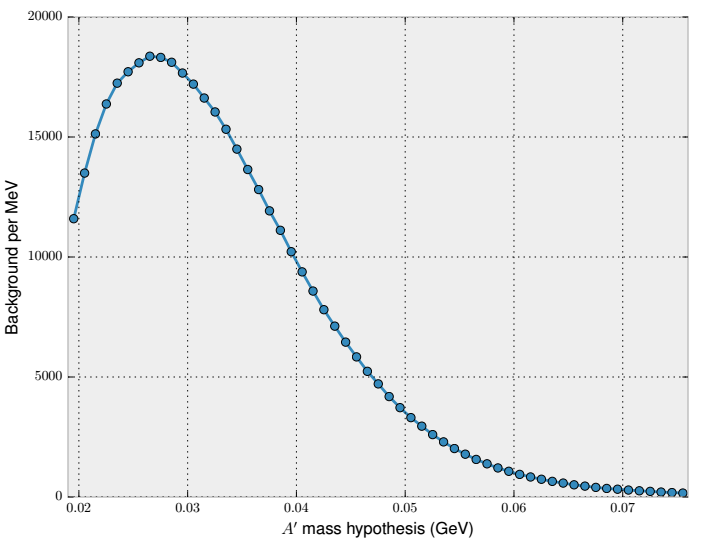
\includegraphics[width=.8\textwidth]{images/bkg_mev.png}
    \caption{The number of background events per MeV at each $A'$ mass hypothesis.}
    \label{fig:background_mev}
\end{figure}
The limits on the coupling strength derived using equation \ref{eqn:eps}
are shown on Fig. \ref{fig:epsilon_upper_limit}.
\begin{figure}[b]
    \centering
    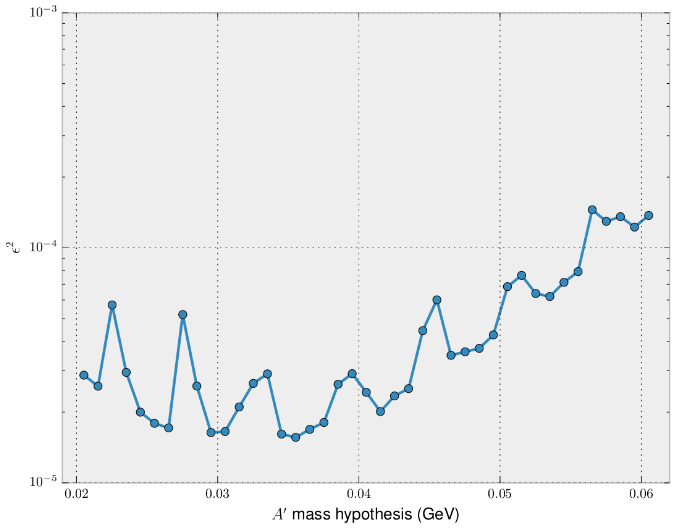
\includegraphics[width=.9\textwidth]{images/final_coupling_upper_limits.png}
    \caption{Upper limits on the coupling strength.}
    \label{fig:epsilon_upper_limit}
\end{figure}





